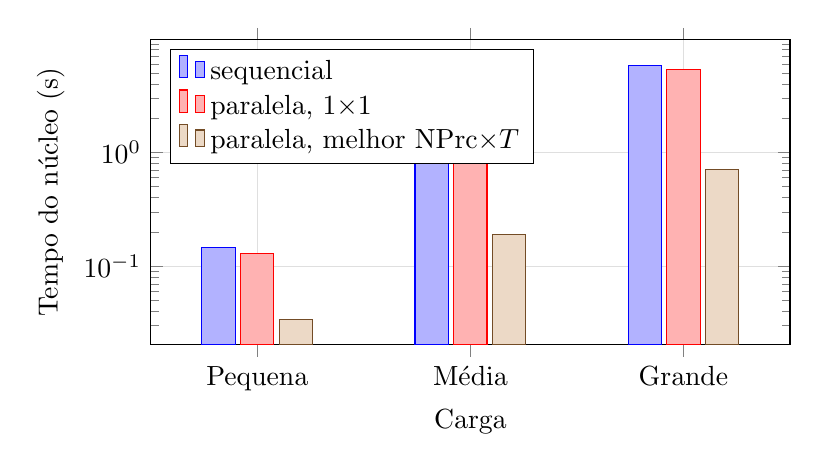
\begin{tikzpicture}
\begin{axis}[
    width=0.8\textwidth, height=0.45\textwidth,
    ybar, bar width=12pt,
    ymode=log, log origin=infty,
    xlabel={Carga}, ylabel={Tempo do núcleo (s)},
    symbolic x coords={Pequena,Média,Grande},
    xtick=data, enlarge x limits=0.25,
    legend pos=north west, legend cell align=left, grid=major, grid style={gray!25},
]
\addplot coordinates {(Pequena,0.145065) (Média,1.679327) (Grande,5.843356)};
\addlegendentry{sequencial}
\addplot coordinates {(Pequena,0.129166) (Média,1.530208) (Grande,5.313043)};
\addlegendentry{paralela, $1{\times}1$}
\addplot coordinates {(Pequena,0.034080) (Média,0.191004) (Grande,0.708088)};
\addlegendentry{paralela, melhor NPrc${\times}T$}
\end{axis}
\end{tikzpicture}
